\documentclass[12pt]{article}
\usepackage{setspace}
\usepackage{graphicx}
\setstretch {1.25} 
\usepackage{geometry}
\geometry{papersize={21cm,29.7cm}}
\geometry{left=2.5cm,right=2.5cm,top=3cm,bottom=3cm}
\usepackage{fancyhdr}
\usepackage{listings}
\usepackage{color}
\definecolor{black}{rgb}{0,0,0}
\definecolor{olivegreen}{RGB}{112,161,71}
\definecolor{lakeblue}{RGB}{0,127,255}
\definecolor{orange}{RGB}{255,139,0}
\definecolor{purple}{RGB}{102,0,255}
\pagestyle{fancy}
\lhead{\author}
\chead{\date}
\lfoot{}
\cfoot{\thepage}
\rfoot{}
\renewcommand{\headrulewidth}{0.4pt}
\renewcommand{\headwidth}{\textwidth}
\renewcommand{\footrulewidth}{0pt}
\usepackage{xeCJK}
\setCJKmainfont{SimSun}
\XeTeXlinebreaklocale “zh”
\XeTeXlinebreakskip = 0pt plus 1pt
\title{OpenGL作业报告\  C类第3题}
\author{夏斐 2012011417}

\date{\today}
\begin{document}
\maketitle
\linespread {1}
\section{实验环境}
本作业在Mac OS X10.8.2系统下用Qt Creator 2.8.2完成,程序框架是Qt GUI,用到了Qt的OpenGL框架,如图所示。为了程序能有更好的用户交互性和为之后的A类和B类作业打基础,之后的作业都用Qt完成。
\begin{center}
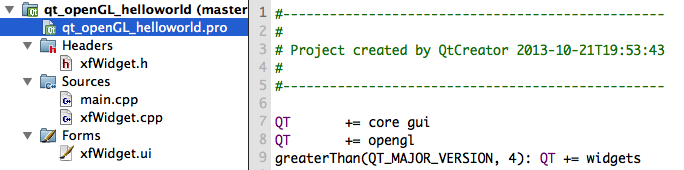
\includegraphics[width = 6in]{environment.png} 
\end{center}
\par
\section{实验原理}
本次作业的原理是在立方体上完成贴图,完成贴图有几个方法,一是直接绑定纹理,在绘制面的过程的同时完成贴图。二是用mipmapping。对于第一种方法,我们需要先载入贴图,在绘制时绑定贴图并且确定映射坐标和映射方式。就可以完成纹理贴图。
\section{实验步骤}
主函数如下,注意到和上一次相比,我们额外增加了glutReshaoefunction,并且在其中设置透视投影矩阵。
\begin{lstlisting}[
language=C++, 
breakatwhitespace=false,
label=lst:helloworld, 
caption=Class xfWidget, 
showspaces=false,
showlines = false,
showstringspaces  = false,
%basicstyle=\ttfamily,
identifierstyle = \color{purple},
stringstyle = \ttfamily,
keywordstyle=\color{lakeblue}\bfseries,
numberstyle = \color{purple}\bfseries,
commentstyle=\color{olivegreen}]
iclass xfWidget : public QGLWidget
{
        Q_OBJECT

public:
        xfWidget( QWidget* parent = 0 );
        ~xfWidget();

protected:
        void initializeGL();
        void paintGL();
        void resizeGL( int width, int height );
        void keyPressEvent(QKeyEvent *e);
        void mousePressEvent(QMouseEvent *e);
        void mouseMoveEvent(QMouseEvent *e);
        void wheelEvent(QWheelEvent *e);
        void loadGLTextures();
private:
        int base;
        float angle;
        GLuint texture[6];
        GLfloat scaling;
        GLfloat xrot, yrot, zrot;
        QPoint lastPos;
        GLfloat posx,posy;


};
\end{lstlisting}
我们放弃了使用Glut,转而使用Qt的widget来完成窗口的管理、和用户的交互,鼠标、键盘等时间的监听等,功能比原来更强大。
\par
载入纹理的过程由下面一段程序实现:
\begin{lstlisting}[
language=C++, 
breakatwhitespace=false,
label=lst:helloworld, 
caption=Load Texture, 
showspaces=false,
showlines = false,
showstringspaces  = false,
%basicstyle=\ttfamily,
identifierstyle = \color{purple},
stringstyle = \ttfamily,
keywordstyle=\color{lakeblue}\bfseries,
numberstyle = \color{purple}\bfseries,
commentstyle=\color{olivegreen},
breaklines=true]
void xfWidget::loadGLTextures()
{
    QString images[6] = {"1.png", "2.png", "3.png","4.png", "5.png", "6.png"};
    glGenTextures(6, &texture[0]);
    for (int i = 0; i < 6; ++i) {
        QImage t;
        QString now = QString("/Volumes/Macintosh HD/dev/OpenGL/OpenGL_Development/qt_openGL_helloworld/images/")+images[i];
        QImage b(now);
        t = QGLWidget::convertToGLFormat(b);
        glBindTexture(GL_TEXTURE_2D, texture[i]);
       glTexImage2D(GL_TEXTURE_2D, 0, 3, t.width(), t.height(), 0, GL_RGBA, GL_UNSIGNED_BYTE, t.bits());
        glTexImage3D(GL_TEXTURE_3D, 0, 3, t.width(), t.height(),0, 0, GL_RGBA, GL_UNSIGNED_BYTE, t.bits());
       //gluBuild2DMipmaps(GL_TEXTURE_2D,GL_RGBA,16,16,GL_RGBA,GL_UNSIGNED_BYTE,t.bits());
        glTexParameteri(GL_TEXTURE_2D, GL_TEXTURE_MIN_FILTER, GL_NEAREST);
        glTexParameteri(GL_TEXTURE_2D, GL_TEXTURE_MAG_FILTER, GL_LINEAR);
    }
}
\end{lstlisting}
\par注意最后三行有一行被注释掉了,这是用于切换贴图模式的,将在效果展示中展示不同的效果。如果都改成NEAREST则不会作线性插值,放大之后会不够清晰,如果是LINEAR则会做线性插值。Mipmaping则相当于选择了另一类的贴图模式。
完成贴图部分用了以下的代码:
\begin{lstlisting}[
language=C++, 
breakatwhitespace=false,
label=lst:helloworld, 
caption=贴图, 
showspaces=false,
showlines = false,
showstringspaces  = false,
%basicstyle=\ttfamily,
identifierstyle = \color{purple},
stringstyle = \ttfamily,
keywordstyle=\color{lakeblue}\bfseries,
numberstyle = \color{purple}\bfseries,
commentstyle=\color{olivegreen}]
    glBindTexture(GL_TEXTURE_2D, texture[5]);
    glBegin(GL_QUADS);
    glTexCoord2f(0.0f, 0.0f); glVertex3f(-1.0f, -1.0f, -1.0f);
    glTexCoord2f(1.0f, 0.0f); glVertex3f(-1.0f, -1.0f,  1.0f);
    glTexCoord2f(1.0f, 1.0f); glVertex3f(-1.0f,  1.0f,  1.0f);
    glTexCoord2f(0.0f, 1.0f); glVertex3f(-1.0f,  1.0f, -1.0f);
    glEnd();
\end{lstlisting}
\par另外值得一提的是,我做了整个系统对于鼠标的响应,	
\begin{lstlisting}[
language=C++, 
breakatwhitespace=false,
label=lst:helloworld, 
caption=mouseevent, 
showspaces=false,
showlines = false,
showstringspaces  = false,
%basicstyle=\ttfamily,
identifierstyle = \color{purple},
stringstyle = \ttfamily,
keywordstyle=\color{lakeblue}\bfseries,
numberstyle = \color{purple}\bfseries,
commentstyle=\color{olivegreen}]
void xfWidget::mouseMoveEvent(QMouseEvent *e)
{
    GLfloat dx = GLfloat(e->x() - lastPos.x()) / width();
    GLfloat dy = GLfloat(e->y() - lastPos.y()) / height();
    if (e->buttons() & Qt::LeftButton) {
        xrot += 180 * dy;
        yrot += 180 * dx;
        updateGL();
    } else if (e->buttons() & Qt::RightButton) {
        xrot -= 180 * dy;
        zrot -= 180 * dx;
        updateGL();
    } else if (e->buttons() & Qt::MiddleButton) {
        posx+=dx*10.24;
        posy+=dy*5.76;
     updateGL();
     }
    lastPos = e->pos();
}
\end{lstlisting}
左键按下和右键按下可以做旋转,中间键按下可以做拖动。滚动滚轮可以缩放。
\section{效果展示}
对六个面采用不同的图案贴图:
\begin{center}
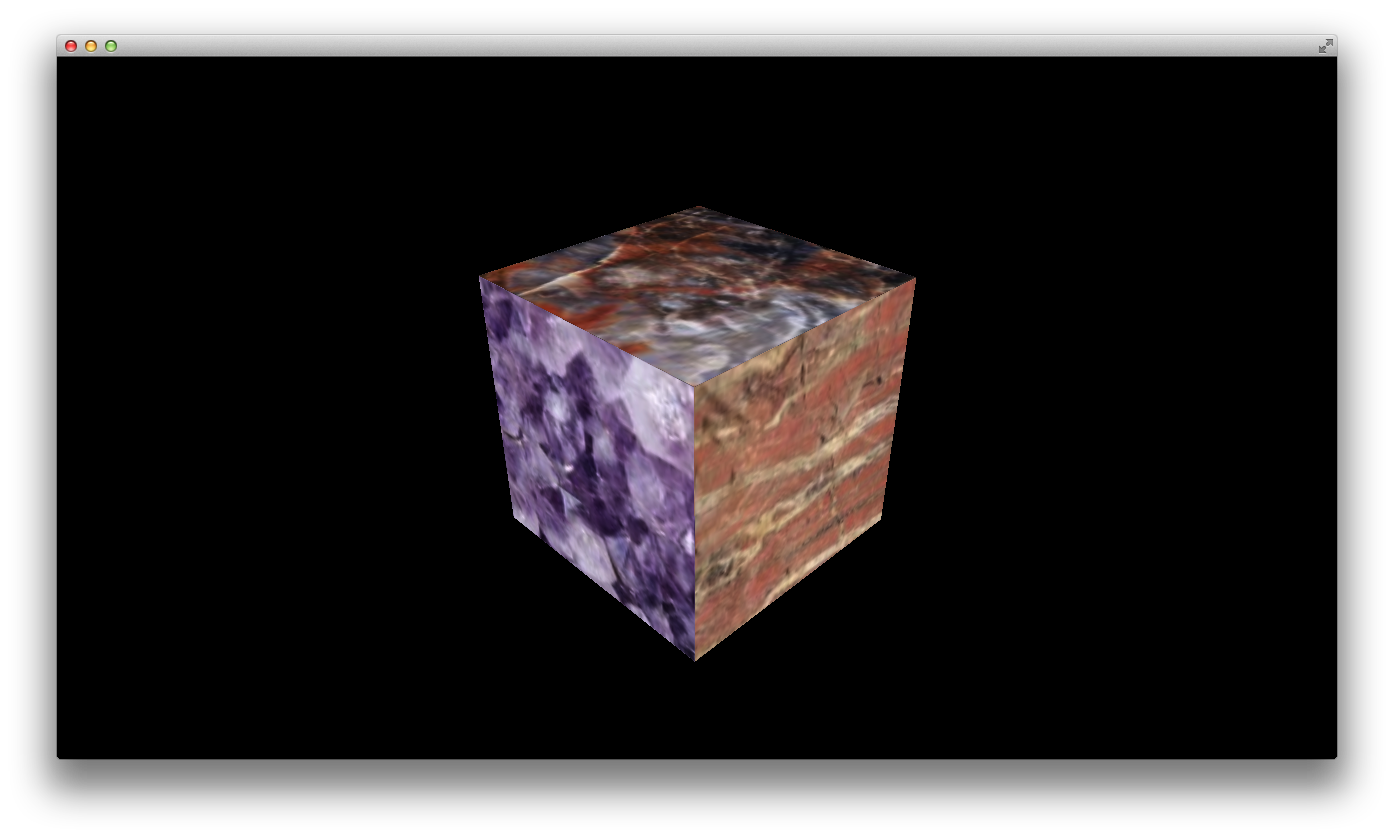
\includegraphics[width = 6in]{1.png} 
\end{center}
用鼠标旋转、移动立方体:
\begin{center}
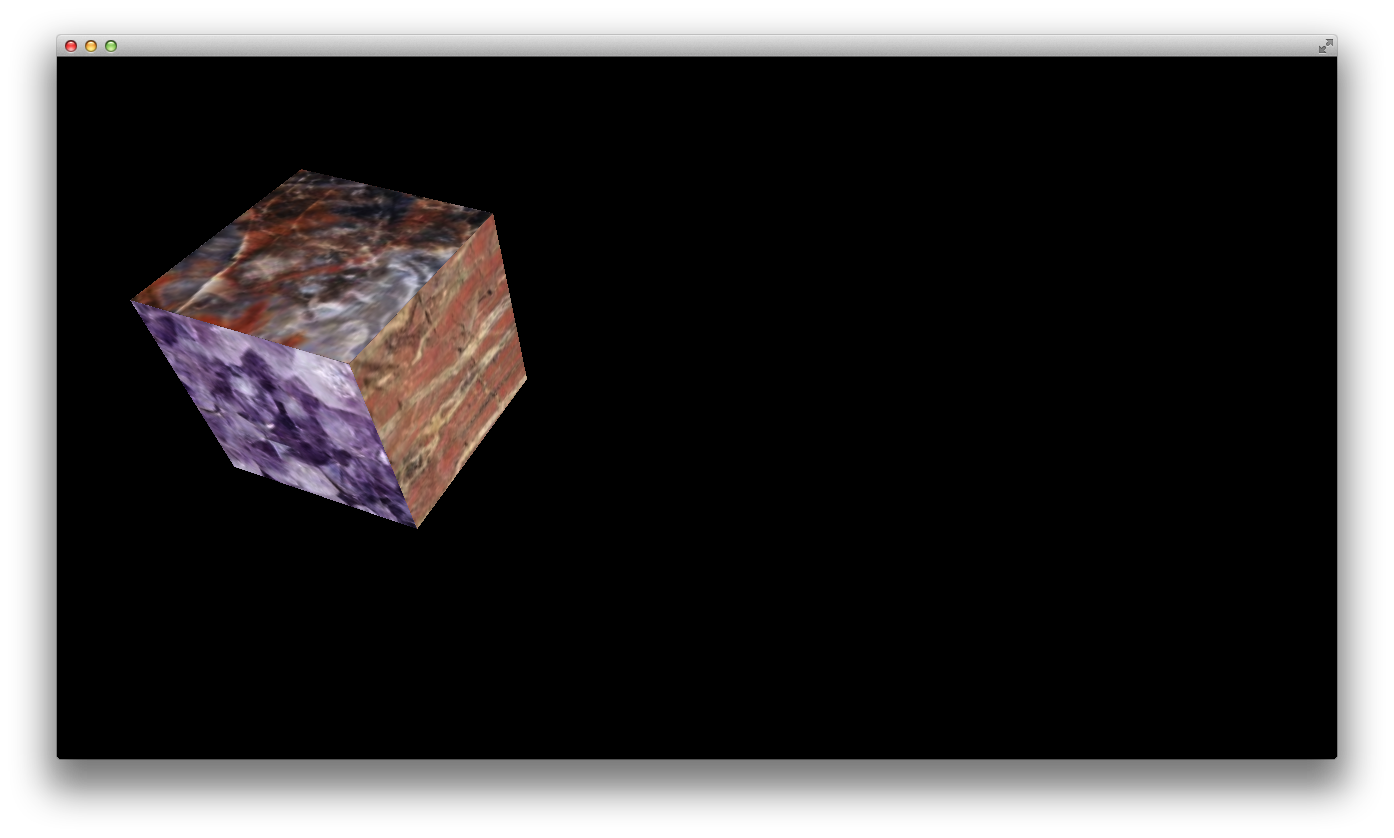
\includegraphics[width = 6in]{2.png} 
\end{center}
贴图时纹理滤波选择线性插值,贴图细腻,放大后不失真:
\begin{center}
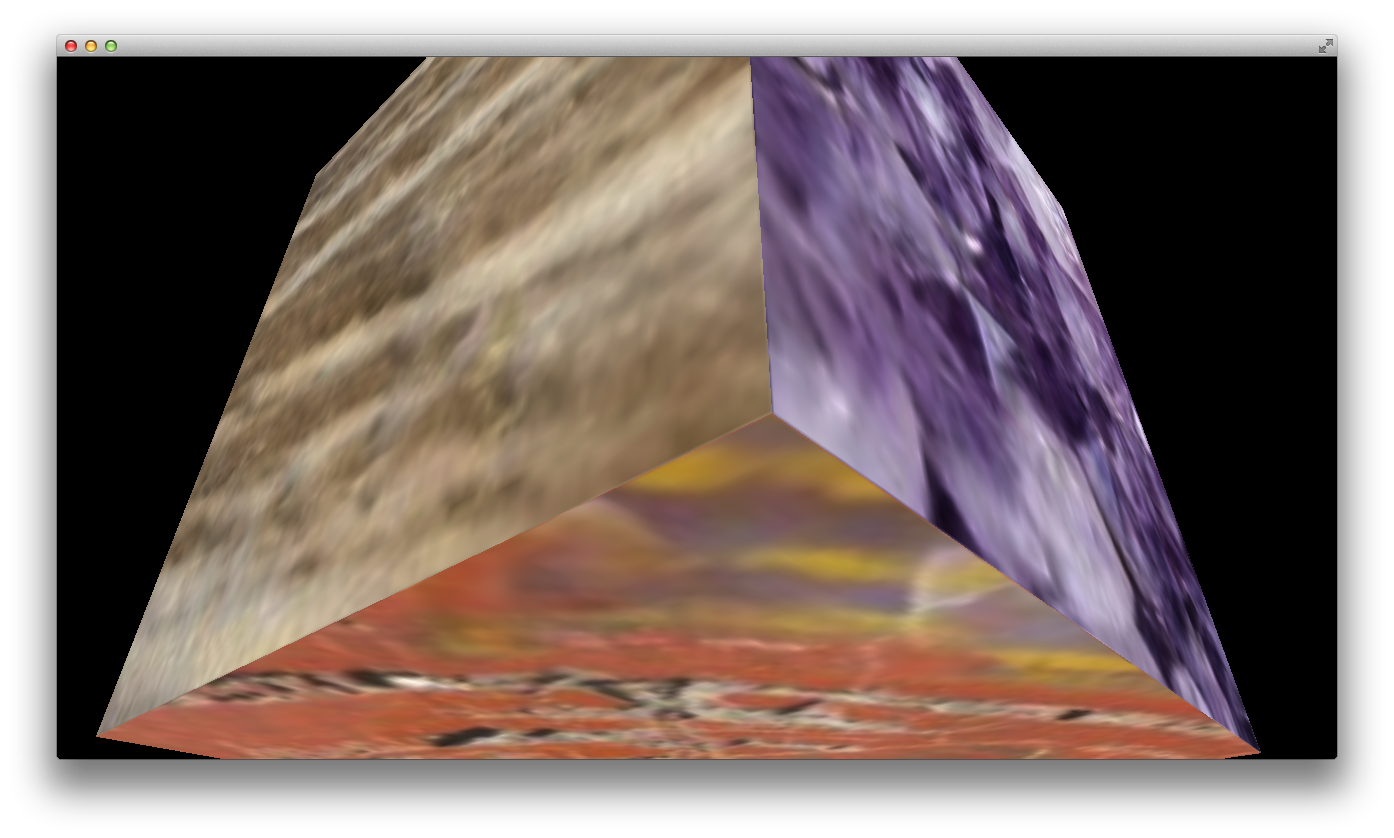
\includegraphics[width = 6in]{3.png} 
\end{center}
贴图时纹理滤波选择NEAREST,贴图放大后可以看到马赛克:
\begin{center}
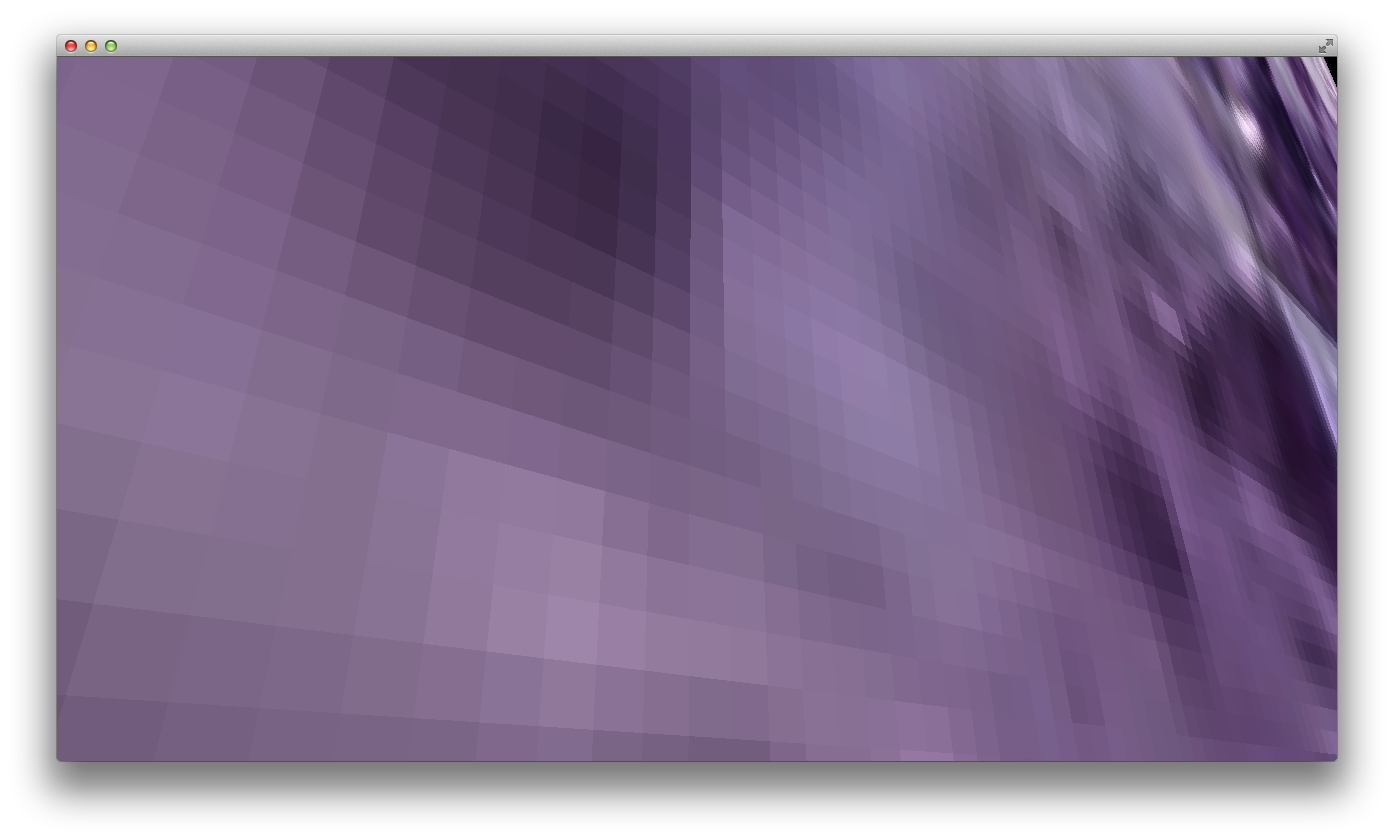
\includegraphics[width = 6in]{5.png} 
\end{center}
采用mipmapping贴图:
\begin{center}
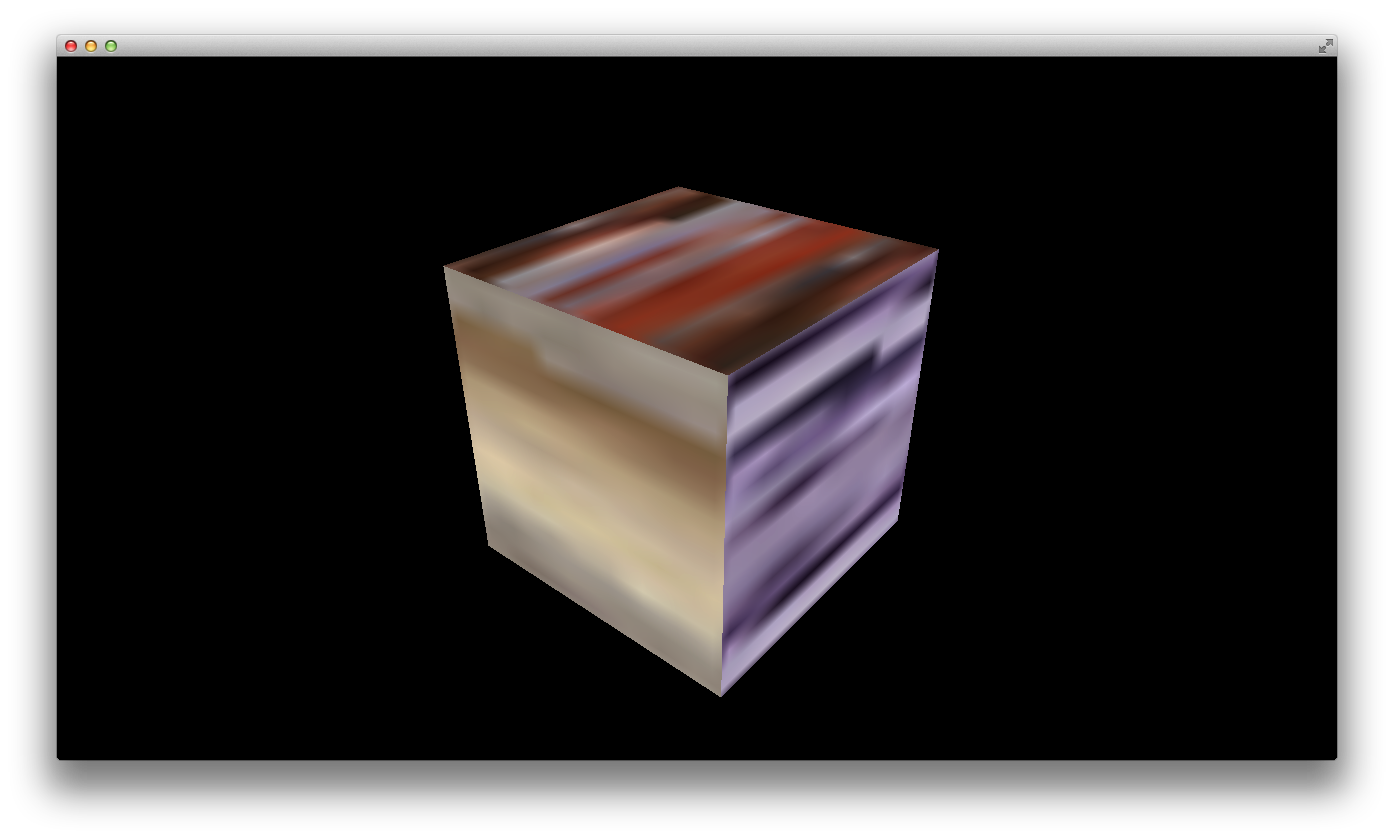
\includegraphics[width = 6in]{4.png} 
\end{center}

\section{参考文献}
[1]来自百度文库 OpenGL入门教程(精)

[2]Nehe OpenGL中文教程
\section{个人信息}
 \noindent
夏斐\\
清华大学 自动化系 2012级\\
手机:(+86)15652799536\\
邮箱:xf1280@gmail.com\\
\end{document}